\documentclass{article}
\usepackage{iclr2018_conference,times}
\usepackage[utf8]{inputenc}
\usepackage{listings}
\usepackage[T1]{fontenc}
\usepackage{hyperref}
\usepackage{url}
\usepackage{subfigure}
\usepackage{booktabs}
\usepackage{amsfonts}
\usepackage{nicefrac}
\usepackage{microtype}
\usepackage{amsmath}
\usepackage{amsthm}
\usepackage{amssymb}
\usepackage{amscd}
\usepackage{mathtools}
\usepackage{enumerate}
\usepackage[ruled,vlined,linesnumbered]{algorithm2e}
\newcommand{\argmax}{\operatorname*{argmax}}
\newcommand{\argmin}{\operatorname*{argmin}}
\newcommand{\var}{\operatorname*{Var}}
\newcommand{\lstd}{\operatorname*{LSTD}}
\newcommand{\diag}{\operatorname*{diag}}
\newcommand{\sgn}{\operatorname*{sgn}}
\newcommand{\lin}{\operatorname*{lin}}
\newcommand{\supp}{\operatorname*{Supp}}
\newcommand{\todo}[2]{{\color{yellow}{#1 TODO: #2}}}
\newcommand*\samethanks[1][\value{footnote}]{\footnotemark[#1]}
\title{Chinese Stock Prediction Using Deep Neural Network}
\newcommand\blfootnote[1]{%
  \begingroup
  \renewcommand\thefootnote{}\footnote{#1}%
  \addtocounter{footnote}{-1}%
  \endgroup
}

\author{Feng Xiaolong  \\
	\texttt{xlfeng886@163.com} \\
}

\newcommand{\fix}{\marginpar{FIX}}
\newcommand{\new}{\marginpar{NEW}}

\iclrfinalcopy
\begin{document}

\maketitle


\newcommand{\Exp}{\mathds{E}}
\newcommand{\Expk}{\mathds{E}_{k}}
\newcommand{\Nat}{\mathbb{N}}
\newcommand{\Ind}{\mathds{1}}
\newcommand{\Rmax}{R_{\rm max}}
\newcommand{\riskyopt}{\succcurlyeq_{\rm ro}}
\newcommand{\cid}{\succcurlyeq_{\rm CID}}
\newcommand{\so}{\succcurlyeq_{\rm so}}
\newcommand{\single}{\succcurlyeq_{\rm sc}}
\newcommand{\ssd}{\succcurlyeq_{\rm ssd}}
\newcommand{\pp}{\mathrel{+}\mathrel{+}}
\newcommand{\Xc}{\mathcal{X}}
\newcommand{\Yc}{\mathcal{Y}}
\newcommand{\Pc}{\mathcal{P}}
\newcommand{\Qc}{\mathcal{Q}}
\newcommand{\Ec}{\mathcal{E}}
\newcommand{\Fc}{\mathcal{F}}
\newcommand{\Gc}{\mathcal{G}}
\newcommand{\Rc}{\mathcal{R}}
\newcommand{\Sc}{\mathcal{S}}
\newcommand{\Ac}{\mathcal{A}}
\newcommand{\Mc}{\mathcal{M}}
\newcommand{\Tc}{\mathcal{T}}
\newcommand{\Vc}{\mathcal{V}}
\newcommand{\Dc}{\mathcal{D}}
\newcommand{\Bc}{\mathcal{B}}
\newcommand{\Hc}{\mathcal{H}}
\newcommand{\A}{\mathcal A}
\renewcommand{\S}{\mathcal S}
\newcommand{\X}{\mathcal X}
\newcommand{\D}{\mathcal D}
\newcommand{\G}{\mathcal G}
\newcommand{\K}{\mathcal K}
\newcommand{\calP}{\mathcal P}
\newcommand{\calI}{\mathcal I}
\newcommand{\barH}{\overline{H}}
\newcommand{\hh}{\hat h}
\renewcommand{\L}{\mathcal L}
\newcommand{\Hyp}{\mathcal H}
\newcommand{\Y}{\mathcal Y}
\newcommand{\B}{\mathcal B}
\newcommand{\C}{\mathcal C}
\newcommand{\F}{\mathcal F}
\newcommand{\E}{\mathbb E}
\newcommand{\W}{\mathcal W}
\newcommand{\Z}{\mathcal Z}
\newcommand{\calE}{\mathcal E}
\newcommand{\calS}{\mathcal{S}}
\newcommand{\calO}{\mathcal{O}}
\newcommand{\Cov}{\textnormal{Cov}}
\newcommand{\V}{\mathbb V}
\newcommand{\Prob}{\mathbb P}
\newcommand{\I}{\mathbb I}
\newcommand{\N}{\mathcal N}
%\newcommand{\M}{\mathcal M}
\newcommand{\tM}{\widetilde{M}}
%\newcommand{\T}{\mathcal{T}}
\newcommand{\balpha}{\boldsymbol \alpha}
\newcommand{\bmu}{\boldsymbol \mu}
\newcommand{\bSigma}{\boldsymbol \Sigma}
\newcommand{\bP}{\mathbf{P}}
\newcommand{\bhP}{\widehat{\mathbf{P}}}
\newcommand{\bT}{\boldsymbol{T}}
\newcommand{\bX}{\boldsymbol{X}}
\newcommand{\bY}{\boldsymbol{Y}}
\newcommand{\bx}{\boldsymbol{x}}
\newcommand{\MV}{\textnormal{MV}}
\newcommand{\hMV}{\widehat{\textnormal{MV}}}
\newcommand{\barmu}{\bar\mu}
\newcommand{\hpi}{\hat\pi}
\newcommand{\tDelta}{\widetilde{\Delta}}
\newcommand{\hmu}{\widehat{\mu}}
\newcommand{\hrho}{\hat\rho}
\newcommand{\heps}{\hat\eps}
\newcommand{\hnu}{\hat\nu}
\newcommand{\trho}{\tilde\rho}
\newcommand{\brho}{\bar\rho}
\newcommand{\hM}{\widehat{M}}
\newcommand{\hN}{\widehat{N}}
\newcommand{\tmu}{\widetilde{\mu}}
\newcommand{\tpi}{\widetilde{\pi}}
\newcommand{\barvar}{\bar\sigma^2}
%\newcommand{\hvar}{\hat\sigma^2}
\newcommand{\tvar}{\tilde\sigma^2}
\newcommand{\R}{\mathcal{R}}
\newcommand{\htheta}{\hat{\theta}}
\newcommand{\hR}{\widehat{\mathcal{R}}}
\newcommand{\tR}{\widetilde{\mathcal R}}
%\newcommand{\var}{\sigma^2}
\newcommand{\invdelta}{1/\delta}
\newcommand{\boldR}{\mathbb R}
\newcommand{\eps}{\varepsilon}
\newcommand{\mvlcb}{\textnormal{\texttt{MV-LCB }}}
\newcommand{\ucb}{\textnormal{\textsl{UCB }}}
\newcommand{\ucbv}{\textnormal{\textsl{UCB-V }}}
\newcommand{\mvlcbt}{\textnormal{\texttt{MV-LCB(t) }}}
\newcommand{\mom}{\textnormal{MoM}}
\newcommand{\me}{\textnormal{ME}}
\newcommand{\mt}{\textnormal{MT}}
\newcommand{\eh}{1/(1-\gamma)}
\newcommand{\ehf}{\frac1{1-\gamma}}


\newcommand{\cvar}{\textnormal{C}}
\newcommand{\hcvar}{\widehat{\textnormal{C}}}
\newcommand{\hvar}{\widehat{\textnormal{V}}}


\newcommand{\avg}[2]{\frac{1}{#2} \sum_{#1=1}^{#2}}
\newcommand{\hDelta}{\widehat{\Delta}}
\newcommand{\hGamma}{\widehat{\Gamma}}




%\newcommand{\todo}[1]{{\bf[#1]}}

\newcommand{\beq}{\begin{equation}}
\newcommand{\eeq}{\end{equation}}

\newcommand{\beqa}{\begin{eqnarray}}
\newcommand{\eeqa}{\end{eqnarray}}

\newcommand{\beqan}{\begin{eqnarray*}}
\newcommand{\eeqan}{\end{eqnarray*}}


\renewcommand{\P}{\mathbb{P}}
\renewcommand{\Pr}{\mathbb{P}}
\newcommand{\Q}{\mathbb{Q}}
%\newcommand{\E}{\mathbb{E}}
\newcommand{\Esp}{\mathbb{E}}
\newcommand{\Var}{\mathbb{V}}
\newcommand{\indic}[1]{\mathbb{I}\{#1\}}
\newcommand{\EE}[1]{\E\left[#1\right]}
%\newcommand{\Prob}[1]{\P\left(#1\right)}
\newcommand{\wh}{\widehat}
\newcommand{\wt}{\widetilde}

\let\R\undefined %sometimes it is defined as something I don't know
\newcommand{\R}{\mathbb{R}}
\newcommand{\Real}{\mathbb{R}}
\newcommand{\Normal}{\mathcal{N}}

\newcommand{\eqdef}{\stackrel{\rm def}{=}}

\newcommand{\cl}[2][ (]{
\ifthenelse{\equal{#1}{ (}}{\left (#2\right)}{}
\ifthenelse{\equal{#1}{[}}{\left[#2\right]}{}
\ifthenelse{\equal{#1}{\{}}{\left\{#2\right\}}{}
}

\newcommand{\inset}[3][C]{
\ifthenelse{\equal{#1}{C}}{{#2}\in\mathcal{#3}}{}
\ifthenelse{\equal{#1}{T}}{{#2}\in{#3}}{}
}

\newcommand{\ESum}[4][C]
{\ifthenelse{\equal{#1}{C}}{\underset{\inset{#3}{#4}}{\sum}#2}{}
 \ifthenelse{\equal{#1}{T}}{\underset{\inset[N]{#3}{#4}}{\sum}#2}{}
\ifthenelse{\equal{#1}{U}}{\overset{#4}{\underset{#3}{\sum}}#2}{}
\ifthenelse{\equal{#1}{X}}{\sideset{}{_{#3}^{#4}}{\sum}#2}{}
\ifthenelse{\equal{#1}{S}}{\sideset{}{_{#3}^{#4}}{\sum}#2}{}
\ifthenelse{\equal{#1}{O}}{{\underset{ (#3,#4)}{\sum}}#2}{}
\ifthenelse{\equal{#1}{I}}{{\underset{#3}{\sum}}#2}{}}

\newcommand{\VF}[2][N]{
\ifthenelse{\equal{#1}{L}}{V^{\pi}_{\lambda} (#2)}{}
\ifthenelse{\equal{#1}{C}}{V{^{\pi} (#2)}}{}
\ifthenelse{\equal{#1}{T}}{V^*_{\bar{\pi}} (#2)}{}
\ifthenelse{\equal{#1}{CO}}{V{^{*} (#2)}}{}
\ifthenelse{\equal{#1}{Mx}}{V^{\pi}_{\infty} (#2)}{}
\ifthenelse{\equal{#1}{Mxo}}{V^{\pi^*}_{\infty} (#2)}{}
\ifthenelse{\equal{#1}{Mn}}{V^{\pi}_{-\infty} (#2)}{}
\ifthenelse{\equal{#1}{Mno}}{V^{\pi^*}_{-\infty} (#2)}{}
}

\newcommand{\Eval}[1][null]{
\ifthenelse{\equal{#1}{null}}{\mathbb{E}}{\mathbb{E}_{#1}}
}

\newcommand{\M}[1][]{
\mathcal{M}_{#1}
}


\newcommand{\qv}[1][null]{
\ifthenelse{\equal{#1}{null}}{Q^*}{Q^{#1}}
}

\newcommand{\T}[1][null]{
\ifthenelse{\equal{#1}{null}}{\mathcal{T}}{\mathcal{T}^{#1}}
}



\newcommand{\subLim}[2]{
\underset{#1\rightarrow#2}{\lim}
}

\newcommand{\Norm}[2][]
{
\left\|#2\right\|_{#1}
}

\newcommand{\bldsym}{\boldsymbol}


% Propositions
%\newtheorem{lemma}{Lemma}
\newtheorem{assumption}{Assumption}
%\newtheorem{corollary}{Corollary}
%\newtheorem{proposition}{Proposition}
%\newtheorem{definition}{Definition}
%\newtheorem{theorem}{Theorem}
%%\newtheorem{proof}{Proof}

% Misc
\newcommand{\TODO}[1]{(\textbf{TODO: {#1}})}
%\newcommand{\remark}[1]{\textbf{Remark #1.}}




\begin{abstract}
	In this research, we study the problem of Chinese stock market forecasting using traditional Neural Network methods, including Deep Feedforward Network, Convolution Neural Network(CNN), Recurrent Neural Network(RNN), Long Short-Term Memory(LSTM) and we have also integrate with the Bi-direction technology. The purpose of this research is not to find a state-of-art algorithm to make the prediction more precise. We focus on the primary method and explore the relationship between architecture and hyper-parameter(including learning rate, variety of activation ,and variety of the output target designed. Due to the advanced of the Deep Learning method in decades, there is much active research in the Time-Serial Analysis domain, but we rarely not sure whether they are work in reality. The real market is a very sophisticated ecosystem, and many accidents may occur, influent the market price. Even there is an efficient market hypothesis from Eugene Fama, but we should not so sure we can control the market by this theoretical analysis. Although we implement the underlying deep neural network architecture, the experiment has a reassuring result with $31.9\%$ accuracy in the eight classes classification task and $68.6\%$ accuracy in the binary classification task.
\end{abstract}
%
\section{Introduction}
\label{sec:introduction}
\subsection{Neural Network and Deep Learning}
Deep learning is a member of machine learning. It is a re-branded name for neural networks—a family of learning techniques that were historically motivated by the way computation works in the brain, and which can be described as learning of parameterized differentiable mathematical functions. The name deep-learning arises from the fact that many layers of these differentiable functions are often attached together. While all of the machine learning can be defined as learning to make forecasts based on past observations, deep learning approaches work by learning to not only predict but also to exactly represent the data, such that it is suitable for the forecast. Given a broad set of desired input-output mapping, deep learning approaches work by feeding the data into a network that produces progressive transformations of the input data until a final transformation predicts the output. The transformations produced by the network are learned from the given input-output mappings, such that each transformation makes it easier to relate the data to the desired label.

While the human designer is in charge of designing the network architecture and training regime, providing the network with a proper set of input-output examples, and encoding the input data in a proper way, a lot of the heavy-lifting of learning the exact representation is performed automatically by the network, supported by the network's architecture.

\subsection{Recent Advances in Deep Learning}
Deep Learning is one of the charming fields in recent years \citep{DBLP:books/daglib/0040158}. The breakthrough of Deep Learning since the success of AlexNet \citep{DBLP:journals/corr/abs-1710-07035} in 2012. Deep Learning is used in the domain of digital image processing to solve severe problems(e.g., image colorization, classification, segmentation, and detection). In that domain,  methods such as Convolutional Neural Networks(CNN) mostly improve prediction performance using big data and unlimited computing resources and have pushed the boundaries of what was possible.

Deep Learning has pushed the boundaries of what was possible in the field of Machine Learning and Artificial Intelligence. Now and then, new and new deep learning techniques are being yielded, exceeding state-of-the-art deep learning techniques. Deep Learning is evolving at a considerable speed, its kind of hard to keep track of the regular advances. In our experiment, we are going to briefly review the basic idea in Deep Learning used in the Chinese stock market.

However, that is not so to say that the traditional Machine Learning techniques \citep{DBLP:journals/tnn/CaoT03},\citep{Kercheval2015Modelling},\citep{DBLP:conf/isnn/ZhaiHH07},\citep{DBLP:journals/isci/ArmanoMM05} which had been undergoing continuous improvement in years before the rise of Deep Learning have become obsolete. But in this paper, we will not review the advantages and disadvantages of each approach. We only focus on the method of Deep Learning applied to the time series problem.

\subsection{Financial Market Prediction and Time Series Analysis}
Modeling and Forecasting of the financial market have been a trendy topic for scholars and researchers. For the efficient markets hypothesis, proposed by Eugene Fama, who is one of the winners of Nobel economics prize in 2013. Although we are not sure about Fama's theory, we should know that Lars peter Hansen shared the same prize at the same time. That mean peoples are confused the question about whether the market could be predicted. Nevertheless, the application for the time series problem is not only used in the market, it also could be used in weather forecasting, statistics, signal processing, pattern recognition, earthquake prediction, electroencephalography, control engineering, astronomy, communications engineering, and primarily in any field applied science and engineering which requires temporal measurements.

Time series analysis comprises methods for analyzing time-series data in order to extract meaningful statistics and other characteristics of the data. Time series forecasting is the application of a model to predict future values based on previously observed values.

\subsection{Dataset Description}
Modern Deep Network method is supported by big data and high-speed data process capability. For the aspect of the data, stock market data is the natural source of the research target. Notably, we dived into the stock market data in China. To find out how the stock market works in China, we should be at first mentioned where the stocks are traded. Thus, we can trade Chinese stocks on the most popular stock exchanges of China: Shanghai Stock Exchange (SSE) and the Shenzhen Stock Exchange (SZSE).

In our experiment, we collect all the daily trade data in the past three decades. The data starts with the first stock released and ends in December 2019. We do not consider the subset of all stocks, but all the stocks data are considered in our experiment. Considering all stocks helps us analyze the internal laws of the Chinese stock market. Because of the difficulty of data processing, we do not use the minute level and hour level data but use the transaction day level data. Although the time scale of the amount of data we use is large, the amount of data at this scale still exceeds 10 million records.

In order to have an intuitive understanding of China’s stock market, we draw the trend chart of the shanghai composite index in Fig.~\ref{fig:SZZZ}.

\begin{figure}[!htp]
	\begin{centering}
		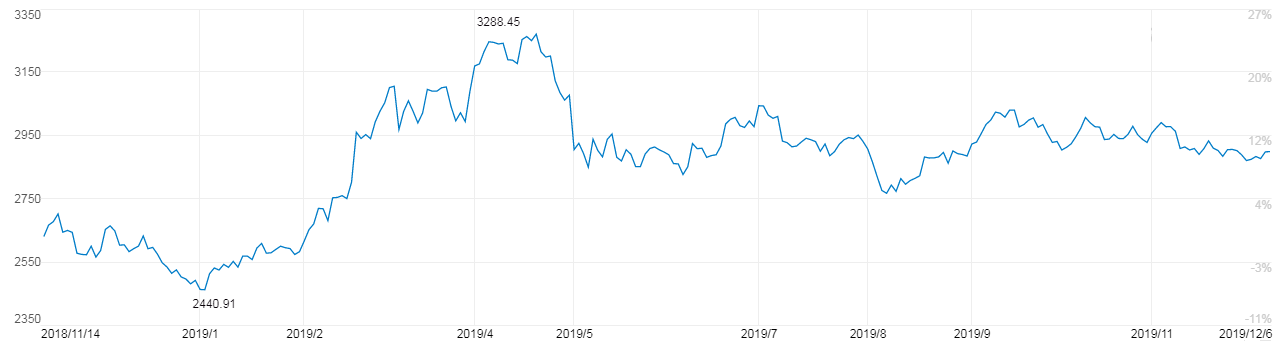
\includegraphics[width=0.8\textwidth]{SZZZ.png}
		\caption{The history shanghai composite index.}
		\label{fig:SZZZ} 
	\end{centering}
\end{figure}

%
\section{Related Work}
\label{sec:Related Work}
Financial time-series prediction is vital for developing excellent trading strategies in the financial market \citep{DBLP:journals/ijbidm/Wang14}. In past decades, it has attracted much attention from researchers of many fields, especially the Machine Learning community \citep{lee1991inferring}. These researches mainly focus on a specific market, e.g., the stock market \citep{DBLP:journals/ijon/Kim03}\citep{DBLP:journals/nca/LiXWCCWMD16}, the foreign exchange market \citep{DBLP:conf/ijcai/LinGA17},\citep{DBLP:journals/eswa/AtsalakisV09}, and the futures market \citep{cheung2019exchange}
,\citep{DBLP:journals/asc/KimAOE17}. Unsurprisingly, this is a holy grail challenge in the finance field due to their irregular and noisy environment.

From the perspective of the learning target, existing researches can be divided into the regression approaches and classification approaches. For the regression approaches, they treat this task as a regression problem \citep{zirilli1996financial},\citep{DBLP:journals/jocs/BollenMZ11}, aiming to predict the future value of financial time-series. While the classification-oriented approaches treat this as a classification problem \citep{DBLP:journals/tois/SchumakerC09},\citep{DBLP:journals/asc/HsiehHY11} focusing on financial time-series classification (FTC).

In most cases, the classification approaches achieve higher profits than the regression ones \citep{DBLP:journals/eswa/HuangYC08}. Accordingly, the effectiveness of various approaches in FTC has been widely explored \citep{DBLP:journals/nca/LiXWCCWMD16},\citep{leung2000forecasting}.
There were also many overview papers on Deep Learning (DL) in the past years. They described DL methods and approaches in significant ways as well as their applications and directions for future research.

In \citep{DBLP:journals/corr/abs-1708-02709}, the researchers talked about DL models and architectures, mainly used in Natural Language Processing (NLP). They showed DL applications in various NLP fields, compared DL models, and discussed possible future trends. Furthermore, in \citep{DBLP:books/daglib/0040158}, the researchers discussed deep networks and generative models in detail. Starting from Machine Learning (ML) basics, pros, and cons for deep architectures, they concluded recent DL researches and applications thoroughly.
%
\section{Advances In Deep Learning}
\label{sec:Advances In Deep Learning}
In this section, we will discuss the leading recent Deep Learning (DL) approaches derived from Machine Learning and brief evolution of Artificial Neural Networks (ANN), which is the most common form used for deep learning.

\subsection{Architecture}
\subsubsection{Multi Layer Perceptron}
As we abandon the brain metaphor and describe networks exclusively in terms of vector-matrix operations. The simplest neural network is called a perceptron. It is simply a linear model is:
\begin{align}
	NN_{Perceptron}(x)=xW + b \\  s.t. \ \ \ \ x \in R^{d_{in}},W \in R^{d_{in}d_{out}},b \in R^{d_{out}}
\end{align}
Where W is the weight matrix, and b is a bias term. In order to go beyond linear functions, we introduce a nonlinear hidden layer, resulting in the Multi Layer Perceptron. A feed-forward neural network with two hidden-layer has the form as :
\begin{align}
	MLP_2(x)=(g^2(g^1(xW^1+b^2)W^2+b^2))W^3\\s.t. \ \ \ x \in R^{d_{in}},W^1 \in R^{d_{in} \times d_{1}},b^1 \in R^{d_1},W^2 \in R^{d_{1} \times d_{2}},b^2 \in R^{d_{2}}
\end{align}
Where g is the nonlinear function, which could be relu, tanh, sigmoid, and so on.
\subsubsection{The CNN architecture}
The convolution-and-pooling (also called convolutional neural networks, or CNNs) architecture, which is tailored to this modeling problem. A convolutional neural network is designed to identify indicative local predictors in a large structure, and to combine them to produce a fixed-size vector representation of the structure, capturing the local aspects that are most informative for the prediction task at hand.

The CNN is, in essence, a feature-extracting architecture. It does not constitute a standalone, useful network on its own, but rather is meant to be integrated into a more extensive network, and to be trained to work in tandem with it in order to produce an end result. The CNN layer's responsibility is to extract meaningful sub-structures that are useful for the overall prediction task at hand.

Convolution-and-pooling architectures evolved in the neural network's vision community, where they showed great success as object detectors—recognizing an object from a predefined category (“cat,” “bicycles”) regardless of its position in the image \citep{DBLP:journals/corr/WangC13b}. When applied to images, the architecture is using 2D (grid) convolutions. When applied to the time series problem, we have mainly concerned with 1D (sequence) convolutions. Because of their origins in the computer-vision community, a lot of the terminology around convolutional neural networks is borrowed from computer vision and signal processing, including terms such as filter, channel, and receptive-field.
We can have an intuitive understanding of CNN from Fig.~\ref{fig:CNN_figure} .


\begin{figure}[!htp]
	\begin{centering}
		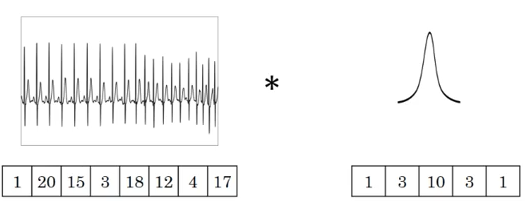
\includegraphics[width=0.8\textwidth]{Conv1D.png}
		\caption{A brief figure for CNN Network Archriculture. This is a 1D Convolution Network, the input in the figure has a data dimension of 8, and the filter has a dimension of 5, and the output data dimension after convolution is 4}
		\label{fig:CNN_figure} 
	\end{centering}
\end{figure}


\subsubsection{The RNN architecture}
As describes RNNs as an abstraction: an interface for translating a sequence of inputs into a fixed sized output that can then be plugged as components in larger networks. Various architectures that use RNNs as a component are discussed.
We use $x_{i:j}$ to denote the sequence of vectors $x_i,\cdot\cdot\cdot,x_j$ . On a high-level, the RNN is a function that takes as input an arbitrary length ordered sequence of $n$ $d_{in}$ dimensional vectors $x_{1:n}=x_1,x_2\cdot\cdot\cdot\cdot x_n$,($x_i \in R^{d_{in}}$) and returns as output a single $d_{out}$ dimensional vector $y_n \in R^{d_{oiut}}$:
\begin{align}
	y_n=RNN(x_{1:n}).\\  s.t.  \ \ \ \ \ x \in R^{d_{in}} ,y_n \in R^{d_{out}}
\end{align}
This implicitly defines an output vector$y_i$ for each prefix $x_{1:i}$ of the sequence x $x_{1:n}$. We denote by $RNN^*$ the function returning this sequence:
\begin{align}
	& y_{1:n}=RNN^*(x_{1:n})\\  & y_i=RNN(x_{1:i})\\ &s.t.  x_i\in R^{d_{in}},y_n \in R^{d_{out}}
\end{align}
The output vector $y_n$  is then used for further prediction. For example, a model for predicting the conditional probability of an event e given the sequence $x_{1:n}$ can be defined as the equation below.
\begin{align}
	p(e=j|x_{1:n})={softmax(RNN(x_{1:n})\cdot W+b)}_{[j]}
\end{align}
The $j_{th}$ element in the output vector resulting from the softmax operation over a linear transformation of the RNN encoding.
\begin{align}
	y_n=RNN(x_{1:n})
\end{align}
We can denote the RNN as the form of recursive as Fig.~\ref{fig:RNN_figure}.

\begin{figure}[!htp]
	\begin{centering}
		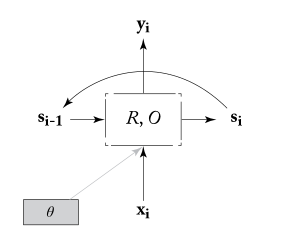
\includegraphics[width=0.4\textwidth]{RNN_recursive.png}
		\caption{A brief figure for RNN Network Archriculture.}
		\label{fig:RNN_figure} 
	\end{centering}
\end{figure}

\paragraph{Bidirectional RNNs (BIRNN)}
A useful elaboration of an RNN is a bidirectional-RNN (also commonly referred to as biRNN) [20 ]. Consider an input sequence $x_{1:n}$. The biRNN works by maintaining two separate states, $s^f_i$, and $s^b_j$ for each input position $i$ . The forward state $s^f_i$ is based on $x_1,x_2\cdot\cdot\cdot\cdot x_i$ , while the backward state $s^b_j$ is based on $x_n,x_{n-1}\cdot\cdot\cdot\cdot x_i$. The forward and backward states are generated by two different RNNs. The first $RNN(R^f,O^f)$ is fed the input sequence $x_{1:n}$ as is, while the second $RNN(R^b,O^b)$ is fed the input sequence in reverse. The state representation $s_i$ is then composed of both the forward and backward states. The output at position $i$ is based on the concatenation of the two output vectors $y_i=[y^f_i:y^b_i]=[O^f(s^f_i):O^b(s^b_i)]$, taking into account both the past and the future. In other words, $y_i$ , the biRNN encoding of the $i_{th}$ word in a sequence is the concatenation of two RNNs, one reading the sequence from the beginning, and the other reading it from the end.
We define $biRNN(x_{1:n},i)$ to  be the output vector corresponding to the $i_{th}$ sequence position:
\begin{align}
	biRNN(x_{1:n},i)=y_i=[RNN^f(x_{1:i}):RNN^b(x_{x_{n:i}})]
\end{align}
The vector $y_i$ can then be used directly for prediction or fed as part of the input to a more complex network. While the two RNNs are run independently of each other, the error gradients at position $i$ will flow both forward and backward through the two RNNs. Feeding the vector $y_i$  through an MLP prior to prediction will further mix the forward and backward signals. Visual representation of the biRNN architecture is given in Fig.~\ref{fig:BINN_figure}.

\begin{figure}[!htp]
	\begin{centering}
		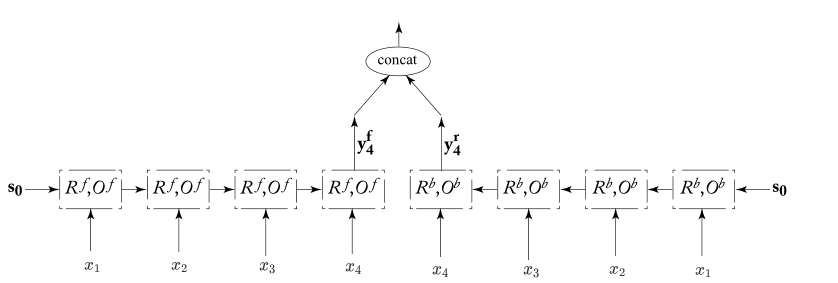
\includegraphics[width=0.8\textwidth]{BIRNN.png}
		\caption{A brief figure for BIRNN Network Archriculture.}
		\label{fig:BINN_figure} 
	\end{centering}
\end{figure}

\paragraph{Multi-Layer(Stacked) RNNs}
RNNs can be stacked in layers, forming a grid \citep{DBLP:conf/nips/HihiB95}. Consider $k$ RNNs, $RNN_1\cdot\cdot\cdot\cdot RNN_k$, where the $j_{th}$ RNN has states $s^j_{1:n}$ and outputs $y^j_{1:n}$. The input for the first RNN is $x_{1:n}$, while the input of the $j_{th}$ $RNN ( j \geq 2 $) are the outputs of the RNN below it $y^{j-1}_{1:n}$, The output of the entire formation is the output of the last RNN, $y^k_{1:n}$. Such layered architectures are often called deep RNNs. A visual representation of a three-layer RNN is given in Fig.~\ref{fig:Three_layers_StckedRNN_figure}..
 
 \begin{figure}[!htp]
 	\begin{centering}
 		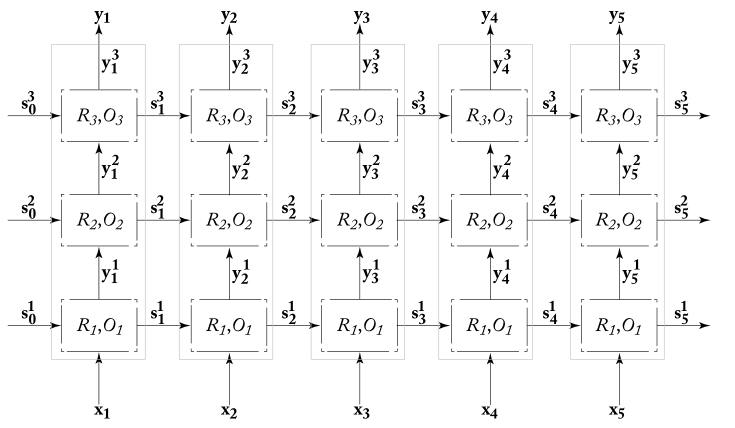
\includegraphics[width=0.8\textwidth]{Three_layere_Deep_RNN.png}
 		\caption{A brief figure for Multi-Layer(Stacked) RNNs Network Archriculture.}
 		\label{fig:Three_layers_StckedRNN_figure} 
 	\end{centering}
 \end{figure}

\paragraph{Simple RNN}
The simplest RNN formulation that is sensitive to the ordering of elements in the sequence is known as an Elman Network or Simple-RNN (S-RNN). The S-RNN was proposed by \citep{DBLP:journals/cogsci/Elman90}. The S-RNN takes the following form:
\begin{align}
	&s_{i}=R_{SRNN}(x_i,s_{i-1})=g(s_{i-1}W^s+x_iW^x+b) \\&y_i=O(s_{i})\\ &s.t. \ \ \  s_i,y_i\in R^{d_{s}},x_i \in R^{d_{x}},W^x \in R^{d_x \times d_{s}},W^s \in R^{d_s \times d_{s}},b \in R^{d_s}
\end{align}
That is, the state $s_{i-1}$ and the input $x_i$ are each linearly transformed, the results are added(together with a bias term) and then passed through a nonlinear activation function $g$ (commonly tanh or ReLU). The output at position $i$ is the same as the hidden state in that position.
\paragraph{Gated Architectures}
The S-RNN is hard to train effectively because of the vanishing gradients problem \citep{DBLP:journals/corr/abs-1211-5063}. Error signals (gradients ) in later steps in the sequence diminish quickly in the back-propagation process and do not reach earlier input signals, making it hard for the S-RNN to capture long-range dependencies. Gating-based architectures, such as the LSTM \citep{hochreiter1997long} and the GRU \citep{DBLP:conf/emnlp/ChoMGBBSB14} are designed to solve this deficiency.
\paragraph{LSTM}
The Long Short-Term Memory (LSTM) architecture \citep{hochreiter1997long} was designed to solve the vanishing gradients problem and is the first to introduce the gating mechanism. The LSTM architecture explicitly splits the state vector $s_i$ into two halves, where one half is treated as “memory cells” and the other is working memory. The memory cells are designed to preserve the memory, and also the error gradients, across time, and are controlled through differentiable gating components —smooth mathematical functions that simulate logical gates. At each input state, a gate is used to decide how much of the new input should be written to the memory cell, and how much of the current content of the memory cell should be forgotten. Mathematically, the LSTM architecture is defined as:
\begin{align}
	s_j=R_{LSTM}(S_{j-1},x_j&)=[c_j:h_j] \\&c_j=f \odot c_{j-1} +i \odot z \\ &h_j=o \odot tanh(c_j)\\&i=\delta (x_j W^{xi}+h_{j-1}W^{hi})\\&f=\delta (x_j W^{xf}+h_{j-1}W^{hf})\\&o=\delta (x_j W^{xo}+h_{j-1}W^{ho})\\&z=tanh(x_j W^{xz}+h_{j-1}W^{hz})\\y_j=&O_{LSTM}(s_j)=h_j\\  s.t. \ \ s_j\in R^{2 \cdot{d_{h}}},x_i \in R^{d_{x}},c_j,h_j,i,f,o,&z \in R^{d_h},W^s \in R^{d_s \times d_{s}},W^{h_0} \in R^{d_h \times d_{h}}
\end{align}
The state at time $j$ is composed of two vectors, $c_j$, and $h_j$, where $c_j$ is the memory component, and $h_j$ is the hidden state component. There are three gates, $i$ , $ f $ , and $o$ , controlling for input, forget, and output. The gate values are computed based on linear combinations of the current input $x_j $and the previous state $h_{j-1}$ , passed through a sigmoid activation function. An update candidate $z$ is computed as a linear combination of $x_j $ and $h_{j-1}$ , passed through a tanha ctivation function. The memory $c_j$ is then updated: the forget gate controls how much of the previous memory to keep $f\odot c_{j-1}$, and the input gate controls how much of the proposed update to keep $i \odot z$. Finally, the value of $ h_j$ (which is also the output $y_j$ ) is determined based on the content of the memory $c_j$, passed through a tanh nonlinearity, and controlled by the output gate. The gating mechanisms allow for gradients related to the memory part $c_j$ to stay high across very long time ranges.
LSTMs are currently the most successful type of RNN architecture, and they are responsible for many state-of-the-art sequence modeling results. The main competitor of the LSTM-RNN is the GRU, to be discussed next.
\paragraph{GRU}
The LSTM architecture is instrumental, but also quite complicated. The complexity of the system makes it hard to analyze and also computationally expensive to work in practice. The gated recurrent unit (GRU) was recently introduced by \citep{DBLP:journals/corr/ChoMGBSB14} as an alternative to the LSTM. It was subsequently shown by \citep{DBLP:journals/corr/ChungGCB14} to perform comparably to the LSTM on several datasets.

Like the LSTM, the GRU is also based on a gating mechanism, but with substantially fewer gates and without a separate memory component.
\begin{align}
	s_j=R_{GRU}(s_{j-1},x_j)&=(1-z) \odot s_{j-1} +z \odot \widetilde s_j \\&z=\delta (x_j W^{xz}+s_{j-1}W^{sz}) \\ &r=\delta (x_j W^{xr}+s_{j-1}W^{sr}) \\ &\widetilde s_j=tanh(x_j W^{xs}+(r \odot  s_{j-1})W^{sg}) \\ y_j=O_{GRU}&(s_j)=s_j \\s.t.. \ \ s_j, \widetilde s_j \in R^{{d_{s}}},x_i \in R^{d_{x}},z,&r \in R^{d_s},W^{xo} \in R^{d_x \times d_{s}},W^s \in R^{d_s \times d_{s}},W^{so} \in R^{d_s \times d_{s}}
\end{align}
One gate ($r$) is used to control access to t()dhe previous state $s_{j-1}$ and compute a proposed update $\widetilde s_j$. The updated state $s_j$  (which also serves as the output $y_j$ ) is then determined based on an interpolation of the previous state $s_{j-1}$ and the proposal $\widetilde s_j$, where the proportions of the interpolation are controlled using the gate z. 
\subsection{Activation Function}
There are some major types of neurons that are used in practice that introduce nonlinearities in their computations. As the list below is the most common activation function :
\begin{enumerate}[(a)]
	\item Sigmoid neurons \citep{DBLP:journals/corr/ElfwingUD17} :
	\begin{align}
		\delta(x)= \frac{1}{1+e^{-x}}
	\end{align}
	\item Tanh neurons \citep{DBLP:journals/corr/abs-1811-03378} :
	\begin{align}
		y=\tag{12}tanh(x)
	\end{align}
	\item ReLU neurons \citep{DBLP:journals/corr/abs-1803-08375} :
	\begin{align}
		y=max(0,x)
	\end{align}
	\item Leaky ReLU neurons \citep{Zhang2017Dilated}:
	\begin{align}
		y=max(0.1x,x)
	\end{align}
	\item Maxout neurons \citep{DBLP:journals/corr/abs-1302-4389}:
	\begin{align}
		y=max(w^T_1x+b_1,w^T_2x+b_2)
	\end{align}
	\item ELU neurons \citep{Clevert2015Fast} :
	\begin{align}
		y=\begin{cases} x &x\ge 0 \\ \alpha(e^x-1) & x<0 \end{cases}
	\end{align}
\end{enumerate}
\subsection{Cost Function and Regularization}
An important aspect of the design of a deep neural network is the choice of the cost function. Fortunately, the cost functions for neural networks are more or less the same as those for other parametric models, such as linear models.
In most cases, our parametric model defines a distribution $p(y|;\theta)$, and we use the principle of maximum likelihood. This means we use the cross-entropy between the training data and the model's predictions as the cost function.

Let $y=y_{[1]}\cdot\cdot\cdot\cdot y_{[n]}$ be a vector representing the true multinomial distribution over the labels $1.....n$, and let $\hat y= \hat y_{[1]}\cdot \cdot\cdot\cdot \hat y_{[n]}$ be the linear classifier’s output, which was transformed by the softmax function, and represent the class membership conditional distribution $\hat y_{[i]}=P(y=i|x)$ . The categorical cross entropy loss measures the dissimilarity between the true label distribution $y$ and the predicted label distribution $\hat y$ , and is defined as cross entropy \citep{DBLP:journals/corr/abs-1909-12830}:
\begin{align}
	L_{cross-entropy}(\hat y,y)=-\sum_{i} {y_{[i]}log(\hat y_{[i]})}
\end{align}
The total cost function used to train a neural network will often combine one of the primary cost functions described here with a regularization term to avoid overfitting issues.
\begin{align}
	\hat\Theta={\underset {\Theta}{\operatorname {arg\,min} }}\,L(\Theta)+\lambda (R(\Theta))\\ \ \ \ ={\underset {\Theta}{\operatorname {arg\,min} }}\,\frac{1}{n}\sum_{i=1}^{n}L(f(x_i;\Theta))+\lambda R(\Theta)
\end{align}
The weight decay approach \citep{DBLP:journals/corr/abs-1907-08931} used for linear models is also directly applicable to deep neural networks and is among the most popular regularization strategies \citep{DBLP:journals/corr/abs-1712-04711}.
\subsection{Optimization}
In order to train the model, we need to solve the optimization problem. A standard solution is to use a gradient-based method. Roughly speaking, gradient-based methods work by repeatedly computing an estimate of the loss $L$ over the training set, computing the gradients of the parameters ‚ with respect to the loss estimate, and moving the parameters in the opposite directions of the gradient. The different optimization methods differ in how the error stimulate is computed, and how “moving in the opposite direction of the gradient” is defined.
While the SGD algorithm can and often does produce good results, more advanced algorithms are also available. The SGD+Momentum \citep{DBLP:journals/corr/abs-1907-07063} and Nesterov Momentum algorithms \citep{DBLP:journals/corr/BotevLB16} are variants of SGD in which previous gradients are accumulated and affect the current update. Adaptive learning rate algorithms, including AdaGrad \citep{DBLP:journals/corr/abs-1806-01811}, AdaDelta \citep{DBLP:journals/corr/abs-1212-5701}, RMSProp \citep{DBLP:journals/corr/Ruder16}, and Adam are designed to select the learning rate for each minibatch, sometimes on a per-coordinate basis, potentially alleviating the need of fiddling with learning rate schedules.
\subsection{Back-propagation}
In the Deep Learning regime, we assumed the function is differentiable, and we can explicitly compute its derivative. In practice, a neural network function consists of many tensor operations chained together, each of which has a simple, known derivative.

Applying the chain rule to the computation of the gradient values of a neural network gives rise to an algorithm called Backpropagation (also sometimes called reverse-mode differentiation). Back-propagation starts with the final loss value and works backward from the top layers to the bottom layers, applying the chain rule to compute the contribution that each parameter had in the loss value.

Nowadays, people will implement networks in modern frameworks that are capable of symbolic differentiation, such as TensorFlow \citep{DBLP:journals/corr/AbadiABBCCCDDDG16} and PyTorch. This means that, given a chain of operations with a known derivative, they can compute a gradient function for the chain (by applying the chain rule) that maps network parameter values to gradient values. When we have access to such a function, the backward pass is reduced to a call to this gradient function.

\subsection{Hyper-parameters}
Deep learning (DL) systems expose many tuning parameters (“hyper-parameters”) that affect the performance and accuracy of trained models. Increasingly users struggle to configure hyperparameters, and a substantial portion of time is spent tuning them empirically. Here we review the most critical part of the hyper-parameters.

\paragraph{Mini-Batch Gradient Descent Hyperparameters}
First, we describe the hyperparameters of mini-batch gradient descent \citep{DBLP:journals/corr/abs-1903-04192}, which updates the network's parameters using gradient descent on a subset of the training data (which is periodically shuffled, or assumed infinite). We'll define the $t_{th} < T$ mini-batch gradient descent update of network parameters ${\theta}$ as :
\begin{align}
	\theta^{(t)} \leftarrow \theta^{(t-1)} -\epsilon_t\frac {1}{B}\sum_{t'=Bt+1}^{B(t+1)}\frac{\partial L(z_{t'},\theta)}{\partial \theta }
\end{align}

where  $z_{t'}$ is example  $t'$  in the training set and the hyperparameters are the loss function $L$, the learning rate at step $t$ $\epsilon _t$, the mini-batch size $B$, and the number of iterations $$T$$. Note that we must define $\theta ^0$, which is also a hyperparameter. For a specific optimization method, as we describe the momentum, it helps to “smooth” the gradient updates using a leaky integrator filter with parameter $\beta$ by
\begin{align}
	\bar g \leftarrow (1-\beta)\bar g+ \beta \frac{\partial L(z_{t'},\theta)}{\partial \theta } 
\end{align}
$\bar g$ can then be used in place of the “true” gradient update in gradient descent. Some mathematically motivated approaches can ensure much faster convergence when using appropriate momentum; however, for pure stochastic gradient descent, standard gradient updates $\beta =1$  with a harmonically decreasing learning rate is optimal.
\paragraph{Model Hyperparameters}
The structure of the neural network itself involves numerous hyperparameters in its design, including the size and nonlinearity of each layer. The numeric properties of the weights are often also constrained in some way, and their initialization can have a substantial effect on model performance. Finally, the preprocessing of the input data can also be essential for ensuring convergence. As a practical note, many hyperparameters can vary across layers.
\begin{enumerate}[(a)]
	\item Number of hidden units
	\item Weight decay, the purpose is to reduce overfitting with the regularization term.
	\item Activation sparsity, it may be advantageous for the hidden unit activations to be sparse. We should consider the type of penalty, L1, L2, or combined L1 and L2.
	\item Nonlinearity, we also should select the type of activation function, as we have described in the previous chapter.
	\item Weight initialization, biases are typically initialized to 00, but weights must be initialized carefully. Their initialization can have a significant impact on the local minimum found by the training algorithm.
	\item Random seeds \citep{DBLP:journals/corr/abs-1806-08295} and model averaging. Many of the processes involved in training a neural network involve using a random number generator (e.g., random sampling of training data, weight initialization.). As a result, the seed passed to the random number generator can have a slight effect on the results. However, a different random seed can produce a non-trivially different model (even if it performs about as well). As a result, it is common to train multiple models with multiple random seeds and use model averaging (bagging, Bayesian methods) to improve performance.
	\item Preprocess input data, the statistics of the input data can have a substantial effect on network performance. Element-wise standardization (subtract the mean and divide by the standard deviation), Principal Component Analysis, uniformization (transform each feature value to its approximate normalized rank or quantile), and nonlinearities such as the logarithm or square root are common.
\end{enumerate}
\paragraph{Hyperparameters Space Exploration}
The number of hyperparameters delineated above indicates that there are a substantial number of choices to be made when creating a neural network learner and that these choices will affect the success and failure of the model. In order to ensure reproducibility of results, a principled approach should be used for setting hyperparameters, or, at the very least, they should be explicitly stated in the model description.

There is some suggestion we can take when we explore the hyperparameters, including coordinate descent, grid search, and random search.
%
\section{Experiments Setup}
\label{sec:Experiments Setup}
\subsection{Tensorflow and Keras}
In our experiment, we use Tensorflow and Keras to build and train the model. Tensorflow is a numeric computing framework and machine learning library. It is the most famous framework for the implementation of Deep Learning. Keras is a high-level neural networks API, written in Python and capable of running on top of TensorFlow, CNTK, or Theano. It was developed with a focus on enabling fast experimentation.  Being able to go from idea to result with the least possible delay is key to doing proper research.

\subsection{feature select}
In the initial version of the data, we have collected 48 features for each stock. In the experiment stage, we find that the number of features does not affect the accuracy too much and reduce to 10 features as we described the dataset above.

To have the intuitive sense of the dataset, here we post a data fragment for the stock code sh600033 in Table~\ref{tab:sh600033TradeData}.

\begin{table}[htbp]
	\centering
	\begin{tabular}{rlrrrrrrrrr}
		\toprule
		\multicolumn{1}{l}{\textbf{Data}} & \textbf{Code} & \multicolumn{1}{l}{\textbf{Open}} & \multicolumn{1}{l}{\textbf{High}} & \multicolumn{1}{l}{\textbf{Low}} & \multicolumn{1}{l}{\textbf{Close}} & \multicolumn{1}{l}{\textbf{Change}} & \multicolumn{1}{l}{\textbf{Volumes}} & \multicolumn{1}{l}{\textbf{MA\_5}} & \multicolumn{1}{l}{\textbf{MA\_10}} & \multicolumn{1}{l}{\textbf{MA\_20}} \\
		\midrule
		2018/2/2 & sh600033 & 3.68  & 3.72  & 3.62  & 3.71  & 0.008152 & 14190281 & 3.748 & 3.783 & 3.741 \\
		2018/2/5 & sh600033 & 3.69  & 3.71  & 3.65  & 3.7   & -0.0027 & 12766982 & 3.726 & 3.772 & 3.741 \\
		2018/2/6 & sh600033 & 3.67  & 3.68  & 3.58  & 3.58  & -0.03243 & 14442600 & 3.684 & 3.751 & 3.7355 \\
		2018/2/7 & sh600033 & 3.63  & 3.64  & 3.55  & 3.56  & -0.00559 & 10008747 & 3.646 & 3.723 & 3.7295 \\
		2018/2/8 & sh600033 & 3.59  & 3.6   & 3.56  & 3.57  & 0.002809 & 7135401 & 3.624 & 3.699 & 3.724 \\
		2018/2/9 & sh600033 & 3.54  & 3.55  & 3.35  & 3.41  & -0.04482 & 16922628 & 3.564 & 3.656 & 3.71 \\
		2018/2/12 & sh600033 & 3.42  & 3.47  & 3.42  & 3.45  & 0.01173 & 5891331 & 3.514 & 3.62  & 3.699 \\
		2018/2/13 & sh600033 & 3.47  & 3.51  & 3.46  & 3.47  & 0.005797 & 5348475 & 3.492 & 3.588 & 3.689 \\
		2018/2/14 & sh600033 & 3.49  & 3.49  & 3.46  & 3.49  & 0.005764 & 3863871 & 3.478 & 3.562 & 3.6765 \\
		\bottomrule
	\end{tabular}%
	\vspace{1em}
	\caption{We report the data fragment for the stock code sh600033 from 2018-2-2 to 2018-2-14.}\label{tab:sh600033TradeData} 
\end{table}

Each row represents one day in one market day, columns from left to right are the date, stock code name, opening price, day high price, day low price, close price, changes, volumes, five days moving average, ten days moving average and twenty days moving average.

\subsection{Label Design}
We divide the experiment into two different problems, binary classification and multiclass classification problem.

In our binary classification problem, we design the output as two output labels. Label $0$ represent the stock in which the price rose, and label $1$ represent the stock price fell. Out network always be ended with a Dense layer with one unit and a sigmoid activation. The output of our network is a scalar between 0 and 1, encoding a probability.

In our multiclass classification problem, we design the output as 8 classes and a single label. Our network ended with a softmax activation so that it will output a probability distribution over the 8 output classes. Categorical crossentropy is the default loss function for our multiclass classification problem. It minimizes the distance between the probability distributions output by the network and the true distribution of the targets. In the Chinese stock market, the maximum daily increase of each stock is 10% and the maximum decline is also 10%. We divide the change from $-0.1$ to $0.1$ into 8 classes.
\begin{align}
	&Class1 \in [-0.1,-0.075) \\ &Class2 \in [-0.075,-0.05) \\&Class3 \in [-0.05,-0.025)\\&Class4 \in [-0.025,0)\\&Class5 \in [0,0.025)\\&Class6 \in [0.025,0.05)\\&Class7 \in [0.05,0.075)\\&Class8 \in [0.075,0.1] 
\end{align}
\subsection{Model design}
we implement the experiment by considering various networ architectures, including MLP, CNN, SimpleRNN, GRU, and LSTM.
\begin{enumerate}[(a)]
	\item In MLP, we mainly use 512 neurons units and following the dropout layer with 0.5 to drop. We also considered different numbers of dense layers in our design.
	\item For CNN, we use the 1D convolution neural layer, with the different filters, kernel size, strides.
	\item For SimpleRNN, LSTM, and GRU: we try different units and activation functions.
	\item For BIRNN, we use the bi-direction trick for all the RNN models.
\end{enumerate}
\subsection{Main hyperparameter design}
\paragraph{Learning rate:} In our experiment, the RMSprop optimizer is the default choice. In some cases, we select some specific learning rate for the RMSprop optimizer, but we let it automated running for most of the cases. We also used the callback function to reduce the learning rate when the validation loss has stopped improving.

\paragraph{Activation function:} we only consider ReLU and tanh as our activation function pool in the nonoutput layers. In the output layer, we use sigmoid for the binary classification problem and  for the multiclass classification problem.

\paragraph{Epochs:} we set the maximum epochs as 200 and use the early stop trick to interrupt training once the target metric being monitored has stopped improving for a various number of epochs.
\paragraph{Lookback and delay steps:} The exact formulation of the stock prediction problem will be given data going as far back as lookback timesteps ( a timestep is one trading day ), we set the lookback trading days as 20 and consider the output in one delayed trading day.
\paragraph{Batch size:} we set the batch size as 1024 in our whole experiment.
\paragraph{Missing data process:} Normally, there are many tricks for missing data process method. For example, fill with average value, last value, min value, max value, or zero. In our experiment, we just fill the missing data as zero.

We list all the architecture in our experiment in Table~\ref{tab:ArchitectureDetail}.

\begin{table}[htbp]
  \centering
   \begin{tabular}{rp{32em}r}
   \multicolumn{1}{l}{ID} & Architecture Detail & \multicolumn{1}{l}{Total Parameters} \\
   \hline
	\\
1  & MLP(512)-LSTM(32)-LSTM(64)-MLP(512)-MLP(8) & 138120 \\
2  & MLP(512)-Bidirectional[LSTM(32)]-MLP(512)-MLP(8) & 183048 \\
3  & [MLP(512)]x6-Flaten-MLP(8) & 1401352 \\
4  & [MLP(512)]x3-Flaten-MLP(8) & 613384 \\
5  & Flatten-MLP(512)-MLP(8) & 117256 \\
6  & MLP(512)-Flaten-MLP(8) & 88072 \\
7  & MLP(512)-Conv1D(32,5)-MaxPooling1D(5)-Conv1D(32,3)-MaxPooling1D-MLP(8) & 91464 \\
8  & MLP(512)-Conv1D(128,3)-MaxPooling1D(5)-Conv1D(128,3)-MaxPooling1D-MLP(8) & 253192 \\
9  & MLP(512)-Conv1D(512,3)-MaxPooling1D(5)-Conv1D(512,3)-MaxPooling1D-MLP(8) & 1584136 \\
10 & MLP(512)-Conv1D(1024,3)-MaxPooling1D(5)-Conv1D(1024,3)-MaxPooling1D-MLP(8) & 5783560 \\
11 & MLP(512)-[Conv1D(32,3),MaxPooling1D(2)]x2-Conv1D(32,3)-MaxPooling1D-MLP(8) & 61800 \\
12 & MLP(512)-[Conv1D(128,3),MaxPooling1D(2)]x2-Conv1D(128,3)-MaxPooling1D-MLP(8) & 302472 \\
13 & MLP(512)-[Conv1D(512,3),MaxPooling1D(2)]x2-Conv1D(512,3)-MaxPooling1D-MLP(8) & 2371080 \\
14 & MLP(512)-GRU(32)-MLP(512)-MLP(8) & 79464 \\
15 & MLP(512)-SimpleRNN(32)-MLP(512)-MLP(8) & 44584 \\
16 & MLP(512)-LSTM(32)-MLP(512)-MLP(8) & 96.904 \\
17 & MLP(512)-LSTM(32)x2-MLP(512)-MLP(8) & 105224 \\
18 & MLP(512)-Bidirectional[(LSTM(32)x2]-MLP(512)-MLP(8) & 207880 \\
19 & MLP(512)-LSTM(32,4)-MLP(512)-MLP(8) & 121864 \\
20 & MLP(512)-Bidirectional[(LSTM(32)x4]-MLP(512)-MLP(2) & 257544 \\
21 & MLP(512)-(LSTM(32)x4-MLP(512)-MLP(8) & 117768 \\
22 & MLP(512)-Bidirectional[(LSTM(32)x4]--MLP(512)-MLP(8) & 257554 \\
23 & MLP(512)-Bidirectional[(LSTM(32)x8]-MLP(512)-MLP(8) & 356872 \\
24 & MLP(512)-Bidirectional[(LSTM(128)x8]-MLP(512)-MLP(2) & 3557896 \\
25 & MLP(512)-Conv1D(512,3)-MaxPooling1D(5)-Bidirectional[LSTM(32)]-MLP(8) & 2899720 \\
26 & MLP(512)-LSTM(32,4)-MLP(512)-BatchNormalization-MLP(8) & 126472 \\
27 & MLP(512)-Bidirectional[(LSTM(32)x4]-MLP(512)-BatchNormalization-MLP(8) & 262664 \\
\bottomrule
\end{tabular}
 \caption{Comparison of all the basic architecture in the experiment. The second column report the architecture details, and the last column report the total number of parameters for each architecture.}\label{tab:ArchitectureDetail} 
\end{table}

In order to have an intuitive understanding of the network architecture, We report the architecture of network number 21 from Table~\ref{tab:ArchitectureDetail} and show the detail in Table~\ref{tab:Architecture21Detail}.

\begin{table}[htbp]
  \centering
    \begin{tabular}{lp{9.94em}r}
    \toprule
    \textbf{Layer (type)          } & \textbf{ Output Shape        } & \multicolumn{1}{l}{\textbf{Parameter Number}} \\
    \midrule
    dense\_1 (Dense)        &  (None, None, 512)    & 2048 \\
    dropout\_1 (Dropout)    &  (None, None, 512)    & 0 \\
    lstm\_1 (LSTM)          &  (None, None, 32)     & 69760 \\
    lstm\_2 (LSTM)          &  (None, None, 32)     & 8320 \\
    lstm\_3 (LSTM)          &  (None, None, 32)     & 8320 \\
    lstm\_4 (LSTM)          &  (None, 32)           & 8320 \\
    dense\_2 (Dense)        &  (None, 512)          & 16896 \\
    dropout\_2 (Dropout)    &  (None, 512)          & 0 \\
    dense\_3 (Dense)        &  (None, 8)            & 4104 \\
    \bottomrule
    \end{tabular}%
	\vspace{1em}
     \caption{We report the architecture detail for the number 21 network in Table~\ref{tab:ArchitectureDetail}, which have 117,768 parameters in total.}\label{tab:Architecture21Detail} 
\end{table}

\subsection{Environment}
Most modern neural network implementations are based on graphics processing units(GPU). GPU is specialized hardware components that were originally developed for graphics applications, but the rise of GPU also dramatically improve the efficiency of neural network training \citep{DBLP:journals/corr/abs-1907-10701}.
Nevertheless, in the daily applications, using GPU is a very high-cost solution, so we also investigated the case of training small neural networks on the CPU. We create some VMs for theses case with the specifications as 6 vCPU and 24G memory.
%
\section{Result and Analysis}
\label{Result and Analysis}
Our experiment result performance is compared with the baseline models. We achieve 0.319 accuracies in the eight classes classification task and achieve 0.686 accuracies in the binary classification task.

In our research work, we have tried more than 200 test cases with different architecture, hyperparameters, and output design. We also give a brief overview of the CPU running time for each model.

\subsection{Architecture Compare}
From the result of the experiment, we find in our designed architecture, and there is a tiny difference in training accuracy, validation accuracy, and test accuracy in the different architecture. We showed the result of the different architecture in Table~\ref{tab:BinaryResult}, and Table~\ref{tab:MultiClassResult}.

In Table~\ref{tab:BinaryResult}, we show the best two models in the binary classification task.
\begin{table}[htbp]
	\centering
	\begin{tabular}{p{20.75em}rr}
		\toprule
		\textbf{Architecture Detail} & \multicolumn{1}{p{4.065em}}{\textbf{Accuracy}} & \multicolumn{1}{p{4.44em}}{\textbf{Valdiation Accuracy}} \\
		\midrule
		MLP(512)-Bidirectional[(LSTM(128)x8]-MLP(512)-MLP(2) & 0.686 & 0.663 \\
		MLP(512)-Bidirectional[(LSTM(32)x4]-MLP(512)-MLP(2) & 0.679 & 0.661 \\
		\bottomrule
	\end{tabular}%
	\vspace{1em}
	\caption{We report the best two architecture in our binary classification problems.}\label{tab:BinaryResult} 
\end{table}
In Table~\ref{tab:MultiClassResult}, we show the best three models in the eight classes classification task.
\begin{table}[htbp]
	\centering
	\begin{tabular}{p{20.75em}rr}
		\toprule
		\textbf{Architecture Detail} & \multicolumn{1}{p{4.065em}}{\textbf{Accuracy}} & \multicolumn{1}{p{4.44em}}{\textbf{Valdiation Accuracy}} \\
		\midrule
		MLP(512)-LSTM(32)-MLP(512)-MLP(8) & 0.319 & 0.306 \\
		MLP(512)-Bidirectional[LSTM(32)]-MLP(512)-MLP(8) & 0.317 & 0.303 \\
		MLP(512)-GRU(32)-MLP(512)-MLP(8) & 0.316 & 0.301 \\
		\bottomrule
	\end{tabular}%
	\vspace{1em}
	\caption{We report the best three architecture in our 8 classes classification problem.}\label{tab:MultiClassResult} 
\end{table}

From the result of the above tables, we observed that:
\begin{enumerate}
	\item The accuracy in the various model only has a tiny difference.
	\item RNN series model, include LSTM, GRU has regularly outperformed the other architecture.
	\item The type of activation does not affect the result, but it impacts the learning progress in the experiment. We find that the ReLU activation function will lead to a smooth learning curve, and tanh activation will lead to a jittery learning curve. Fig.~\ref{fig:activation_compare} shows a comparison between the two types of activation function.
	\begin{figure}[!htp]
		\begin{centering}
			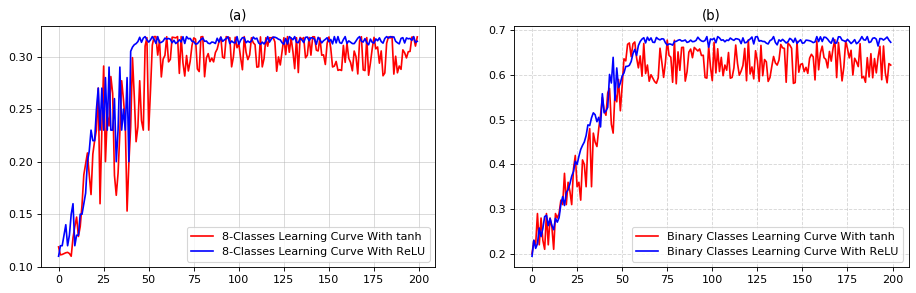
\includegraphics[width=1.0\textwidth]{tanh_relu.png}
			\caption{The learning curve compares for tanh and relu activation neurons. The left figure shows the learning curve for the network MLP(512)-LSTM(32)-MLP(512)-MLP(8) in the 8 classes classification task. The right figure shows the learning curve for the network MLP(512)-Bidirectional[(LSTM(128)x8]-MLP(512)-MLP(2) in the binary classification task. 
}
			\label{fig:activation_compare} 
		\end{centering}
	\end{figure}
	\item the learning rate does not impact the result as we use the RMSprop as the default optimizer.
\end{enumerate}
\subsection{Computation Time in CPU}
We have created more than 30 VMs with the specifications as 6 vCPU and 24G memory to test the running time per epoch in every architecture. The result showed that different network architectures have considerable differences in CPU running time. In practice, we suggest selecting the simpler architecture and only loss a little accuracy of the result.

We report the best top three inTable~\ref{tab:TopEfficientArch} and the worst top three inTable~\ref{tab:WorstEfficientArch}.
\begin{table}[htbp]
	\centering
	\begin{tabular}{p{20.75em}rrr}
		\toprule
		\textbf{Architecture Detail} & \multicolumn{1}{p{9.25em}}{\textbf{CPU running time per epoch(second)}} & \multicolumn{1}{p{4.065em}}{\textbf{Accuracy}} & \multicolumn{1}{p{6.315em}}{\textbf{Validation Accuracy}} \\
		\midrule
		Flatten-MLP(512)-MLP(8) & 400   & 0.3005 & 0.3012 \\
		MLP(512)-[Conv1D(32, 3), MaxPooling1D(2)]*2-Conv1D(32, 3)-MaxPooling1D-MLP(8) 970 0.314 0.285 & 970   & 0.314 & 0.285 \\
		MLP(512)-SimpleRNN(32)-MLP(512)-MLP(8) & 1163  & 0.3005 & 0.3013 \\
		\bottomrule
	\end{tabular}%
	\vspace{1em}
	\caption{We reported the best top three efficient architecture when CPU was used with comparable accuracy.  }\label{tab:TopEfficientArch} 
\end{table}

\begin{table}[htbp]
	\centering
	\begin{tabular}{p{20.75em}rrr}
		\toprule
		\textbf{Architecture Detail} & \multicolumn{1}{p{9.25em}}{\textbf{CPU running time per epoch(second)}} & \multicolumn{1}{p{4.065em}}{\textbf{Accuracy}} & \multicolumn{1}{p{6.315em}}{\textbf{Validation Accuracy}} \\
		\midrule
		MLP(512)-Conv1D(1024, 3)-MaxPooling1D(5)-Conv1D(1024, 3)-MaxPooling1D-MLP(8) & 102828 & 0.314 & 0.285 \\
		MLP(512)-Bidirectional((LSTM(128)x8)-MLP(512)-MLP(8) & 85571 & 0.301 & 0.304 \\
		MLP(512)x6-Flaten-MLP(8) & 29872 & 0.311 & 0.3 \\
		\bottomrule
	\end{tabular}%
	\vspace{1em}
	\caption{We reported the worst three architecture when CPU was used with similar accuracy.}\label{tab:WorstEfficientArch} 
\end{table}


\section{Discussion and Future Work}
\label{Discussion and Future Work}
Focusing on the stock market in China, we propose the basic Deep Neural Network to get a comparable result for the stock prediction problem. According to the competent performance of models in the practical application, deep neural network methods have strong implications for investors as well as the entire stock market in China. The financial industry might integrate deep neural network prediction result in traditional prediction models to make better decisions. This is an interesting filed and promising direction in behavioral finance.

This study has inevitable limitations, which might be exciting directions in future work. We prepare to explore some potential directions to improve accuracy.

First, we could implement different structure of feature extractor, such as Transformer \citep{DBLP:journals/corr/JaderbergSZK15}, BERT\citep{DBLP:journals/corr/abs-1810-04805}, GAN\citep{DBLP:conf/nips/KrizhevskySH12}.

Second, other modern neural network architecture may be worth to try like AlexNet\citep{DBLP:journals/corr/abs-1710-07035}, GoogLeNet\citep{DBLP:journals/corr/SzegedyLJSRAEVR14}, VGG19\citep{simonyan2017very}, ResNet\citep{DBLP:journals/corr/HeZRS15}.

Third, the attention mechanism \citep{DBLP:journals/access/LiuW19} can be introduced to handle long-term dependency, which cannot be handled by RNN.

Forth, our hyper-parameter is only designed by heuristic, and if we have the formal policy for hyperparameter search, the result should be better than the current result. The coordinate descent, grid search, and random search policy are the suggested method for the future hyperparameters fine-tune.

Fifth, the deep reinforcement learning method is also well suited for the stock market prediction problem.

Sixth, the feature of the current dataset should not be enough if we use a robust network architecture; we should consider more features for each stock. Furthermore, some other conditions should also be beneficial, such as the international market trends, the future market price, the exchange market price, and the emotion status in the social network.

\bibliography{CSPUDNN}
\bibliographystyle{CSPUDNN}
\newpage
\appendix
 
%
\end{document}

